\documentclass[twocolumn]{article}
\usepackage{graphicx}

\title{Enhancing household survey microdata accuracy using machine learning: project plan}
\date{}
\author{Nikhil Woodruff}

\begin{document}

\maketitle

\section{Project outline}

Tax-benefit policy is the set of rules that determine tax liabilities and benefit entitlements, deciding the allocation of nearly half of GDP in the United Kingdom alone. When policymakers, think-tanks or academic institutions propose changes to tax-benefit policy, they often use mathematical models to estimate the impact of such changes. The dominant approach to modelling tax-benefit policy is \emph{microsimulation}. Microsimulation models are combined of two parts: a model of policy logic that can compute taxes and benefits for a given household under current and proposed changes, and dataset representative of a target population, on which the policy model is executed. Given that the most common population of interest is the private household population in a country, most microsimulation models use a household survey dataset as their input. The most common of these surveys is the Family Resources Survey (FRS).

The accuracy of microsimulation models is crucial to their utility. Policy logic is easier to verify, since it is specified in detail by legislators. However, household surveys can often fail to be truly representative of the population. We know that this is the case, because we have access to other datasets which are both quantitatively different (in the distributions of shared variables) and more likely to be correct (due to better administration processes or higher population coverage). For example, the Survey of Personal Incomes (SPI) is a random sample of HMRC's Real Time Information computer-based database of personal tax and income data. Both the FRS and SPI contain the annual dividend income of respondents, but the total dividend income in the FRS is aound 40\% of the total in the SPI.\cite{frs_capital_income} Similarly, the Department for Work and Pensions estimated in 2008 that the FRS excluded 26\% of the Severe Disablement Allowance recipient population that should have been included in a representative sample of the UK household sector.\cite{dwp_110}

Approaches to improving the accuracy of household survey data (up to the accuracy of administrative data) as used in microsimulation have been limited and largely unsuccessful. This can lead analyses to use separate datasets in order to answer separate policy impact questions. For example, if a tax policy raises taxes on dividends to fund a universal cash transfer, analysis which uses the SPI to estimate tax revenues, and the FRS to estimate the percentage of households better off under the policy, will be biased because the FRS under-represents the dividend-holding population, while the SPI accurately represents it.

This project will aim to answer the question of \emph{how much can machine learning improve the accuracy of household surveys}. It will survey the current approaches used to improve the accuracy of household surveys (not limited to the U.K.). It will implement various different methods (including the current state-of-the-art) and evaluate their performance at reducing the gap between the FRS and administrative data when used to answer questions about the U.K. household population. These methods will include:
\begin{itemize}
    \item Percentile-based adjustment of data values.
    \item Gradient-descent based methods to reweight household records.
    \item Matching-based methods to impute data across surveys.
    \item Random forest-based imputation of data across surveys.
    \item Distributional random forest-based imputation.
\end{itemize}
\section{Project plan}

The project has been split into several sections for simplicity. Each task, numbered below, is shown in the Gantt chart in Figure \ref{gantt_chart}.

\subsection{Literature survey}

\begin{enumerate}
    \item The literature survey will analyse current approaches to improving survey microdata accuracy, primarily from across the United States, Europe and the U.K. 
\end{enumerate}

\subsection{Calibration}

This section will evaluate the extent by which reweighting (using gradient descent) can outperform changing data values according to percentiles in adminstrative data.

\begin{enumerate}
    \setcounter{enumi}{1}
    \item Implement percentile adjustment on the FRS using the SPI.
    \item Implement gradient-descent-based reweighting.
    \item Benchmark methods against each other.
    \item Write up validation results and conclusions.
\end{enumerate}

\subsection{Imputation}

In this section, I will evaluate the performance of novel and SOTA methods for imputation, the process of adding in data in a survey with data from another survey.

\begin{enumerate}
    \setcounter{enumi}{5}
    \item Implement matching.
    \item Implement random forest imputation.
    \item Implement distributional random forest imputation.
    \item Benchmark methods against each other.
    \item Write up validation results and conclusions.
\end{enumerate}

\subsection{Application}

Under this section, I will apply the calibration and imputation methods together on the FRS, assessing any change in accuracy.

\begin{enumerate}
    \setcounter{enumi}{10}
    \item Gather calibration data for the FRS.
    \item Apply a calibration method to the FRS.
    \item Apply an imputation method to the FRS from other household surveys.
    \item Apply reweighting together with imputation for the SPI income variables.
    \item Evaluate any change in accuracy on SPI income variables.
    \item Benchmark the enhanced FRS against the original on unseen targets.
    \item Write up the FRS enhancement process and performance.
\end{enumerate}

\subsection{Review}

This phase is the final review stage, ensuring the project report is complete.

\begin{enumerate}
    \setcounter{enumi}{17}
    \item Review the final report.
\end{enumerate}

\begin{figure}[ht]
    \centering
    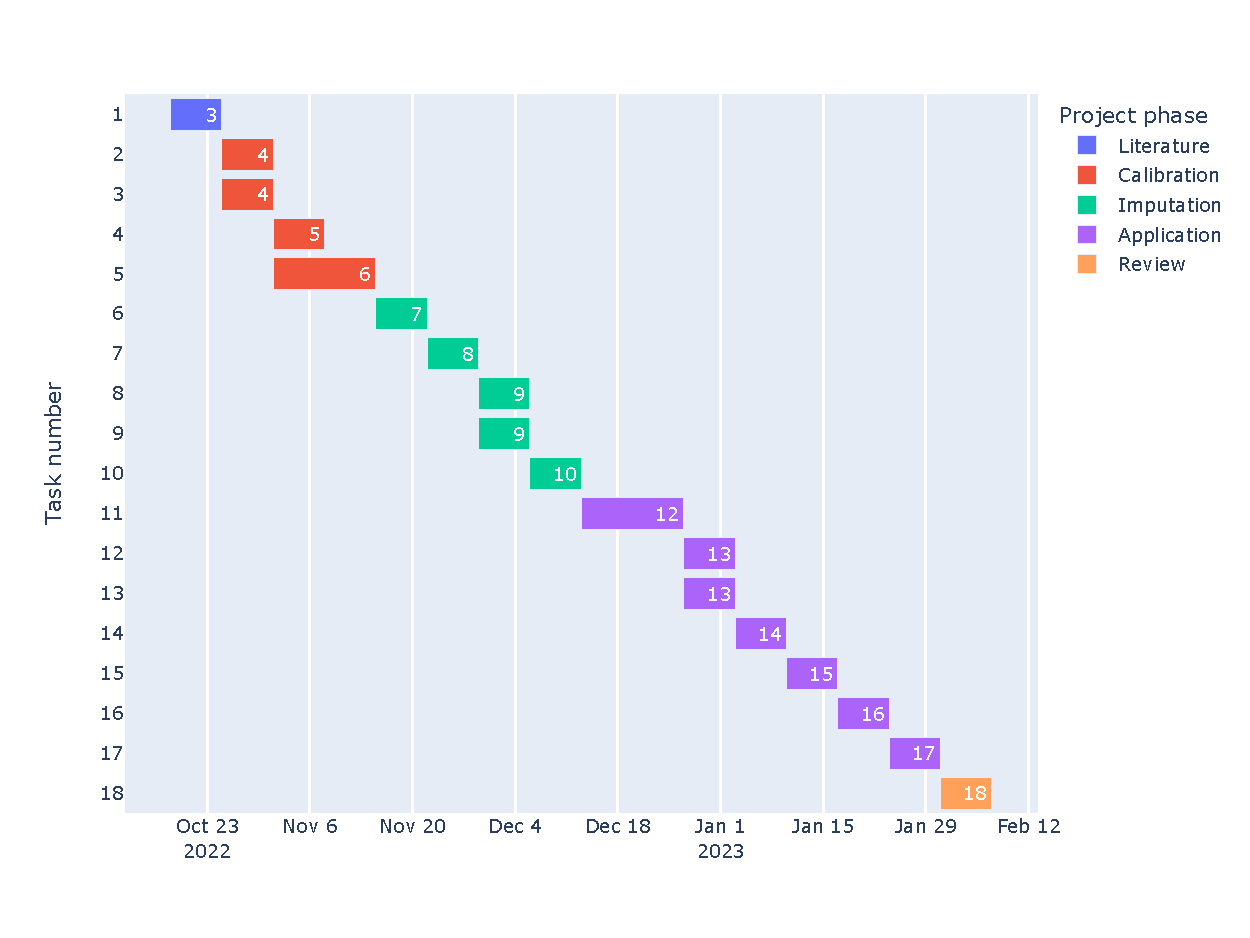
\includegraphics[width=1.0\textwidth]{gantt_chart.pdf}
    \caption{Gantt chart with project milestones}
    \label{gantt_chart}
\end{figure}

\bibliography{../references}
\bibliographystyle{plain}

\end{document}
